%0       1         2         3         4         5         6         7         8
%2345678901234567890123456789012345678901234567890123456789012345678901234567890
%
%
%
% \subsection{Science Goals}
% \subsection{Software Goals}
% \subsubsection{Adaptive Mesh Refinement}
% \subsubsection{Particles}
% \subsubsection{Hyperbolic and Elliptic Methods}
% \subsubsection{Dynamic Task Scheduling}
%    CHARM++
%
%    large-scale demonstration

%    particle precision
%    grid position
%    timestepping
% REQUIREMENTS: scope of library / framework
%    capabilities
%       physics
%          hyperbolic
%          elliptic
%          ray-tracing?
%       AMR
%       Particles
%       performance
%       parallel scaling
%       data structure scaling
%       ease of use
%       dynamic scheduling
%       aggressive minimization of global communication
%       I/O
%       fault tolerance
%       adaptivity
%       extensibility
% DESIGN: software organization and data structures
%    high-level design
%       OOP
%       components
%          Simulation, Control, Parallel, Task
%          Amr, Patch: stores the AMR hierarchy
%          Fields, Particles, Array: for storing data
%          Block, Fluxes: for computing / communicating data
%          Performance, Error, Parameters, Memory
%             globally-accesible functions; components in
%             aspect-oriented programming paradigm; not sufficiently
%             important to use AspectC, but techniques (primarily
%             using templates) usable
%          Method [Analysis] [Visualize]
%             hooks to user code; multiple methods permitted,
%             selectable and scheduled at run-time
%       user interface
%          External, User
%       application-driven
%    data structures
%
% ALGORITHMS: and how problems solved
%    AMR
%    particles
%    parallelization
%    load balancing
%    fault tolerance
% IMPLEMENTATION
%    Languages: C++, C99, UPC, OpenMP
%    Libraries: HDF5, MPI
%    Frameworks: CHARM++, OpenCL
%    TRAC
%      wiki used for design
%      tickets for tasks and documenting defects
%    Subversion
%    unit testing
%    regression testing
%      lcatest
%      correctness, single-thread performance, weak and strong parallel scaling
%          shallow and deep problems
%      lcaperf
%    software reviews

% Requirements
%    
% Design
% Implementation




%=======================================================================
\documentclass[14pt,letter]{article}
%=======================================================================

% INCLUDE DEVELOPMENT TEXT

\newcommand{\devel}[1]{\textbf{#1}}

% EXCLUDE DEVELOPMENT TEXT

% \newcommand{\devel}[1]{}


%=======================================================================
% Document layout
%=======================================================================

\setlength{\topmargin}{0.0in}
\setlength{\oddsidemargin}{0.0in}
\setlength{\evensidemargin}{0.0in}
\setlength{\textwidth}{6.0in}
\setlength{\textheight}{9.0in}

%=======================================================================
% Packages
%=======================================================================

\usepackage{wasysym}
\usepackage{epsfig}
\usepackage{url}

%=======================================================================
% Commands
%=======================================================================

\newcommand{\cello}{\textsf{Cello}}
\newcommand{\enzo}{\textsf{Enzo}}
\newcommand{\lcaperf}{\textsf{lcaperf}}
\newcommand{\lcatest}{\textsf{lcatest}}

\newcommand{\code}[1]{\textsf{#1}}

\newcommand{\note}[1]{\devel{\eighthnote\ \textit{#1} \\}}
\newcommand{\pargraph}[1]{\devel{\P\ \textbf{#1} \\}}

\newcommand{\todo}{\devel{$\circ$}}
\newcommand{\done}{\devel{$\bullet$}}
\newcommand{\halfdone}{\devel{\textcolor{gray}{$\bullet$}}}

\newcommand{\PROJECT}{\cello}

\newcommand{\TITLE}[3]{
\title{ {\huge \PROJECT\ #1}  \\ \vspace{0.1in}
     {\small Document Version: \textbf{#3}} \vspace{-0.1in}
    }
\author{      #2 \\
        Laboratory for Computational Astrophysics\\
        University of California, San Diego}
\maketitle}

%=======================================================================


\usepackage{natbib}

%=======================================================================

\begin{document}

\tableofcontents
%\Large
% \renewcommand{\pargraph}[1]{}

\nocite{StSh09} % Scalability challenges for massively parallel {AMR} applications
\nocite{WiHy03} % Enhancing scalability of parallel structured {AMR} calculations
\nocite{GuWi06} % Parallel clustering algorithms for structured {AMR}
\nocite{BuGh08} % Towards adaptive mesh {PDE} simulations on petascale computers
\nocite{BaBu09} % MPI on a million processors


%=======================================================================
\TITLE{A Software Framework for Extreme Adaptive Mesh Refinement}{James Bordner}{$Rev$}
%=======================================================================

\section{PROJECT SUMMARY}  \label{s:summary}

\pargraph{Proposal}
We propose to develop a new software framework for adaptive mesh
refinement (AMR) that allows application developers to write
multiphysics applications for simulating phenomena on an extreme range
of spacial and temporal scales, and that require an extreme amount of
computation, memory, and storage (petascale and beyond).
%
\note{data parallel plus optional pipelined task parallelism}
%
\pargraph{data structure scope summary}
Our basic data structure is a fully parallel distributed octree, with
associated arrays and particles, supporting both Eularian, Lagrangian,
and hybrid methods such as Particle Mesh (PM).
%
\pargraph{parallelization strategy}
Multiple parallelization technologies can be used, including MPI, UPC,
OpenMP, or CHARM++.  Hybrid approaches will also be supported, with
MPI or UPC for distributed memory data and UPC or OpenMP for shared
memory data.
%
\pargraph{extreme scalability}
Extreme scalability will be obtained by aggressively localizing the
individual patch / block problems; this will help control scalability issues
related to limited floating-point precision and range, as well as
reducing the need for global synchronization and reduction operations.
% integer range
%
@@@@@@@@@@@@@@@@@@@@@@@@@@@@@@@@@@@@@@@@@@@@@@@@@@@@@@@@@@@@@@
\pargraph{load balancing}
Dynamic load balancing will be hierarchical, both to better adapt to
the hierarchical nature of extreme scale computational platforms, and
to allow flexibility in load balancing frequency and metrics at different
levels.
%
\pargraph{fault tolerance}
Fault tolerance and software resilience are crucial factors at extreme scales,
since it has been observed that frequency of failures is proportional to
the number of sockets.
due to the reduced MTTI (mean time to interrupt) , since the probability that hardware component, operating system, library, or application component fails Unfortunately, approaches to fault tolerance are still 
%
\pargraph{I/O}
Disk I/O is also a crucial factor for petascale 

\pargraph{availablity}
We plan to make this framework publicly available for scientific research use.

\pargraph{motivation}
Our motivation for this project is to develop a new AMR framework with emphasis on extreme scalabilityboth in the parallel and data structure sense.
Advantage: designing with extreme scale in mind from the beginning.

% DOE buzzwords
% \url{http://www.er.doe.gov/ASCR/WorkshopsConferences/MathTalks/M\_wright.pdf}

\note{highlight contributions: improved tree-based AMR}
\note{distributed datastructure}
\note{multilevel parallelism}
\note{flexible data storage in memory}
\note{dynamic execution and communication scheduling}

Runtime management system:
\begin{enumerate}
\item Partition applications
\item Allocate resources
\item Balance load
\item Manage communication
\end{enumerate}

% AMR \\
% applied mathematics\\
% collaborative software environments\\
% computer science technologies\\
% exascale \\
% extreme scale\\
% failure avoidance \\
% failure effects avoidance \\
% fault tolerance\\
% GPU \\
% HPC \\
% memory hierarchy\\
% multicore\\
% multiphysics \\
% multiscale \\
% one-sided communication\\
% performance tuning\\
% petascale \\
% PGAS \\
% research goals\\
% resilient software \\
% UPC \\
% virtual processes \\
% 
% \url{http://diversity.doe.gov/documents/Writing\_Winning\_Proposals.pdf}
% 
\begin{verbatim}
intro: compelling, organization goals and success, relevence to agency
problem statement--needs assessment
    purpose
    beneficiaries
    what is being done
    what we will do
objectives: table with direct items
development plan
   chart with timelines
   decision points
   milestones
   tasks
methods and design
    use flow charts and diagrams to break up text
    justify course of action
    highlight innovative features
past experience
management approach
  quality control
  emphasize performance management
  technological systems in place
\end{verbatim}

\begin{verbatim}
Overriding design goals
Extreme parallel scalability
Extreme data structure scalability

Innovative ideas
hierarchical load balancing
separate scheduling of communication and computation
pipelining computational methods to increase parallelism
AMR: patch coalescing
AMR: targeted refinement by 4, 8 with backfill
only store local coordinates for particles
only store local patch connectivity
gang scheduling for GPU support
fault tolerance @@@
multiple parallelization technologies with flexible hybrid support

refined  / borrowed ideas
fully distributed AMR datastructure
patch block registers for improved computing / user interface flexibility
communication flux registers (Chombo) for communication
guard cells allocated when needed
localized fully-adaptive time-stepping (no global reductions) (refined)
\end{verbatim}


\begin{verbatim}
preliminary results
good references critical; only give great references
use rfp keywoards
quality control
sustainability--what happens when money ends
deliverables: software, research papers, workshop/training
sales document not technical manual
visit agency web site for similar funding
make benefits clear
write for evaluators
justify and support all claims
active voice: strong subjects and active verbs
first paragraph sentence conveys topic
65 characters per line
duplicate information instead of cross reference
use graphics and tables
short text with bullets
stay on topic
\end{verbatim}

%=======================================================================
\section{EXTREME SCALING ISSUES} \label{s:issues}
%=======================================================================

\begin{verbatim}
Hardware-related parallel scaling issues
   software resiliency
   AMR-specific parallel scaling issues
   AMR data structure scaling issues
\end{verbatim}

%=======================================================================
\section{Extreme Scaling Issues} \label{s:scaling}
%=======================================================================


\note{load balancing summary}

We will use a hierarchical dynamic load balancing approach, with
support for balancing with respect to multiple metrics (memory use,
computational load, etc.) for different hierarchical computational
components (node, socket, etc.), with different rebalancing
frequencies for different levels.

%=======================================================================
\section{EXISTING AMR FRAMEWORKS} \label{s:review}
%=======================================================================

\begin{verbatim}
 http://people.sc.fsu.edu/~tomek/AMR/index.html
 *   Adaptive Mesh Refinement Software for Hyperbolic Conservation Laws, Marsha Berger
 * Adaptive Mesh Refinement and Parallel Computing, John A. Trangenstein, Mathematics Department, Duke University.
 * Amrita, James Quirk.
 * AMR1D, a simple adaptive mesh refinement code for solving the one-dimensional Euler equations on an unstructured grid.
 * AMRCART, The AMRCART MHD Code, Rolf Walder.
 * AMRCLAW, Adaptive Mesh Refinement + CLAWPACK. AMRCLAW is a joint project between Randy LeVeque and Marsha Berger.
 * AMRMHD3D, 3-D AMR code with FCT MHD solver.
 * AMROC, Blockstructured Adaptive Mesh Refinement in object-oriented C++, Ralf Deiterding.
 * AMRPoisson, Solving Poisson's Equation using Adaptive Mesh Refinement (AMR), Computational Fluid Dynamics, Dept. of Mechanical Engineering, U.C. Berkeley.
 * ARMS, 3-D AMR code with FCT MHD solver.
 * BEARCLAW, general purpose software package for solving time-dependent partial differential equations, Sorin Mitran, Applied Mathematics Program, The University of North Carolina at Chapel Hill.
 * BSAMR, Block Structured Adaptive Mesh Refinement, Daniel D. Wake, College of Engineering, UC Davis.
 * Cactus, The Cactus Code Server, Max Planck Institute for Gravitational Physics (Albert Einstein Institute), Max Planck Society.
 * Cart3D, Michael J. Aftosmis, Numerical Aerospace Simulation (NAS) Division Systems, NASA Ames Research Center
 * CTH, 3-D multi-material Eulerian AMR code from Sandia (export controlled).
 * Enzo, Cosmological Simulation Code, Laboratory for Computational Astrophysics, UCSD.
 * FEMLAB, FEM with automatic error control for two-dimensional convection-diffusion-absorption problems.
 * FLASH, multi-physics 3-D octree AMR parallel code.
 * Gerris Flow Solver, incompressible fluid flow with arbitrarily complex solid boundaries and adaptive mesh refinement, Stephane Popinet.
 * GrACE, Grid Adaptive Computational Engine, Manish Parashar.
 * NIRVANA, 3-D MHD AMR code, Udo Ziegler.
 * PARAMESH, 3-D octree AMR parallel code.
 * RACOON, Institute for Theoretical Physics I, University of Bochum.
 * SARA, A Solution Adaptive Remeshing Algorithm for structured grids, Dave Banks, Center for CFD, Dept. of Mech & Aero Eng, UC Davis.
 * Solution-Adaptive Grids, W. M. Keck Foundation CFD laboratory, University of Michigan.
 * SUUMA3D, Scalable Unstructured Mesh Algorithms and Applications, MCS ANL. 
\end{verbatim}

There are numerous AMR frameworks, libraries, and applications, each
with different design goals and decisions, data structures, AMR
algorithms, parallelization strategies, and parallel performance and
scaling.  Perhaps the top three most successful and closely related to
our proposed effort are PARAMESH (\cite{MaOl00} \nocite{OlMa05}
\nocite{Ol06}), Chombo (\cite{wwwchombo} \cite{CoGr09}), and SAMRAI
(@@@).  Other notable software include Clawpack (@@@), GrACe / DAGH
(@@@), ALPS (\cite{BuBu09}), and Carpet (@@@).


GADGET-2: Preeminent cosmological TreeSPH simulation code
DAGH (1998)

%-----------------------------------------------------------------------
\subsection{PARAMESH}
%-----------------------------------------------------------------------

\nocite{wwwparamesh}
\nocite{MaOl00} % PARAMESH requested references
\nocite{OlMa05}
\nocite{Ol06}

The PARAMESH software was developed at the NASA Goddard Space Flight
Center and Drexel University.

Octree-based AMR


Due to a loss of funding PARAMESH can no longer be supported.

%-----------------------------------------------------------------------
\subsection{Chombo}
%-----------------------------------------------------------------------

\nocite{wwwchombo}
\nocite{CoGr09}

Chombo is in active development by the Applied Numerical Algorithms
Group of Lawrence Berkeley National Lab.  Its high-level design
consists of five loosely-coupled components based on a mathematical
decomposition: \code{BoxTools} for set calculus on point sets and
unions of rectangles, \code{AMRTools} for interprocess communication
between AMR levels, \code{AMRTimeDependent} for advancing the solution
using adaptive timestepping, \code{AMRElliptic} for the
multigrid-based solution of elliptic AMR problems, \code{EBTools} for
embedded boundaries, and \code{ParticleTools} for particle processing
(not available in the current 3.0 version, according to the website
due to re-engineering of the component).

CHOMBO is very scalabale, and designed to run both hyperbolic and
elliptic problems on 10,000 processors.

Berger-Rigoutsos 

\note{Chombo parallel data distribution}

Distributed data in \code{LayoutData}, \code{BoxLayoutData}, and 
\code{LevelData} containers. [ch7 design]

\note{Chombo load balancing}
Provides load balancing algorithm, as well as allowing user to provide their own.
[ch7 design]


%-----------------------------------------------------------------------
\subsection{SAMRAI}
%-----------------------------------------------------------------------

[2001]


good scaling for numerical and data communication
poorer scaling in adaptive meshing and communication schedule construction 


%=======================================================================
\section{CELLO REQUIREMENTS / SCOPE} \label{s:requirements}
%=======================================================================

\begin{verbatim}
 multi-level
 multi-physics
 Enzo II: built on framework, but independent
 equations
    hyperbolic conservation
    elliptic
    local physics
 user-supplied functions
    single-patch advance
    inter-resolution constraints
    refinement criteria
 performance
    serial performance
    parallel performance
    parallel scaling
    memory usage
 data structures
    breadth
    depth
 software resiliency
 hardware support
    multicore
    gpu / accelerators
    distributed and / or shared memory
 parallel technology support
    directly: CHARM++, MPI, UPC, OpenMP, + combinations
    indirectly: GPU / accelerator
 I/O
 what we do not do
    visualization
    analysis utilities
\end{verbatim}

%=======================================================================
\section{CELLO DESIGN} \label{s:design}
%=======================================================================

\begin{verbatim}
Components
   Method
   Control, Parallel, Task
      dependencies known: patch can advance when its neighbor data is known
   Amr, Array, Patch, Tree, Node 
   Fields, Particles
   Block, Fluxes, ItBlock*
   Memory, Performance
   Error
   Monitor, Portal
   Simulation
   Parameters
\end{verbatim}

\begin{verbatim}
General goals

extreme parallel scalability
extreme data structure scalability
  breadth: number of grid patches
  depth: number of AMR hierarchy levels

for parallel scalability: aggressive minimization of
  synchronization and collective operations
``localize'' problem as much as possible
  For each patch, only store patch, location information for
    neighboring patches (``ghost patches''), and ancestors for octree
  patch-local adaptive timestep control
    prevents rapidly evolving feature in one localized region of
      domain from determining timestep elsewhere
facilitate dynamic load balancing, dynamic scheduling of
  communication and computation
maximize data structure flexibility
dynamically optimize data structure parameters to hardware
  during run time
for algorithmic scalability: aggresively minimize dependencies
  of fp and integer precision on data structure size
related to ``localization'' of tasks
  particle positions stored using local coordinate system with
    origin at patch corner
  absolute patch coordinates not stored, only position relative
    to neighbors
     global coordinates only needed for initialization
     only need mesh width and timestep size for advancing
     not needed for restarts
     can still be computed dynamically
     localization an option--not needed for smaller problems
     absolute particle positions / grid locations may be needed
       for some output, e.g. global particle analysis
     in that case low precision
     still scaling issues relative to depth
      neighbor location
\end{verbatim}

%=======================================================================
\section{Project data structures and algorithms}
%=======================================================================

%-----------------------------------------------------------------------
\subsection{Dynamic task scheduling}
%-----------------------------------------------------------------------
\note{task scheduling summary}

Given that tasks are acceptably load-balanced across process, the
tasks must be schedule for execution.  The @@@


We will use dynamic scheduling of tasks assigned to a processes, since
it @@@  Dynamic scheduling is more suitable than static scheduling for
heterogeneous sized tasks, non-regular communication dependencies @@@

\note{task scheduling details}

After tasks are distributed among processing elements, the next
decision is how to schedule tasks among processing elements.  Two main
approaches are static and dynamic.  Static scheduling is preferred
when workload is evenly mapped to processing components, and when
there are relatively few tasks per process.  We will use dynamic
scheduling, since workload (communication as well as computation) per
task varies between tasks.

\note{CHARM++ summary} 
Our approach will be well-mapped to CHARM++,
which is a fault-tolerant message-driven parallel programming
framework.  CHARM++ also provides dynamic load balancing through task
migration, and provides fault tolerance through its built-in disk (or
memory + disk) checkpoint / restart mechanism.

\note{implementation in CHARM++}
Implementation of AMR for a hyperbolic problem, a parallel task, or
CHARM++ ``chare'', would correspond to advancing a numerical method or
sequence of methods one timestep on a single grid patch block.  The
exchange of guard cell data would correspond to CHARM++ messages.
This implementation would allow a block to advance one timestep as
soon as all of its guard cell data is available.

\note{non-CHARM++ implementation}

We also plan to develop our own scheduler, for several reasons.  One,
to schedule communication in addition to computation, to help hide
latency through prefetching.  Second, to take advantage of
hierarchical hardware components (node, socket, core...)  Third, to
remove any hard dependencies on any single parallel technology.

%-----------------------------------------------------------------------
\subsection{hierarchical dynamic load balancing}
%-----------------------------------------------------------------------

Dynamic load balancing is well known to be a crucial operation for
extreme scalability in general, and for extreme adaptive mesh
refinement in particular.

A common approach of rebalancing SAMR hierarchies based on octrees is
to linearize the data structure using a Morton or Hilbert type
space-filling curve, and partition the nodes among processes by
dividing the linearized structure into $N_P$ evenly sized pieces.
This approach works well if the work and memory usage is roughly equal

for each node, and if the global \code{MPI\_AllGather} of long
integers on $N_C$ cores is acceptable \footnote{\cite{BuGh08}
  indicates $N_C$ cores, though we believe with a hybrid programming
  approach their global reduction could be reduced to an even more
  scalable $N_P$ MPI processes}.  However, we anticipate that this
approach will not be sufficient for a general-purpose extreme AMR
framework for several reasons.
%
One, adaptive timestepping is required for efficient ``deep'' AMR
problems, but that scales the work load for a given node by a
non-constant factor of roughly $2^k$ for level $k$.
%
Two, particle distributions among nodes may not be uniform, affecting both memory and computational loads.
%
Three, array patches may be differently sized, if we use our ``coalesced patches'' enhancement to reduce the AMR tree node count.  
%
Four, performance of physics methods on a patch is not necessarily
uniform, due to, e.g., localized subcycling of stiff methods, front
tracking methods, etc.  The first three issues, and possibly the
fourth, could be addressed by dynamically weighting nodes before
partitioning them among processes, but that would require additional
global communication to perform the reduction.
%

Lastly, we suspect that linearizing the workload artificially
restricts the flexibility of data movement allowed (along one
dimension instead of three), creating more communication traffic
during task migration.  than in not be optimal in terms of the amount
of data that needs to be redistributed during each rebalancing step,
since it restricts workload along a single dimension, whereas the
actual workload is typically distributed along three or four
dimensions (three spacial and one time).

Since we suspect that a space-filling curve approach is only effective
for a strict subset of AMR problems we wish to support, we will
explore two ideas for dynamic load balancing, including ``hierarchical
load balancing'', and a new approach we call ``deliberate
overcompensation''.

\note{load-balancing: hierarchical} 
%
By \textit{hierarchical load balancing} we mean rebalancing tasks
between higher levels (nodes or supernodes) independently from
rebalancing between lower levels (socket or cores).  The idea of
hierarchical task scheduling and load balancing has been known for at
least 15 years (\cite{AhGh94}, but is not commonly used for AMR
frameworks.

This will have several advantages over more traditional
non-hierarchical load balancing.  First, rebalancing at different
levels could be based on different metrics, e.g. memory usage for
rebalancing between nodes, and computational load for rebalancing
between sockets.  This will be particularly useful for AMR problems,
because memory is the crucial metric we want to keep balanced at the
node level, yet we want to balance computational time at lower
hardware platform levels to keep computational elements busy.  Second,
rebalancing frequencies at different levels can be decoupled,
rebalancing less frequently at the upper node levels where rebalancing
is more costly, and where load tends to take longer to become
unbalanced.

\note{load-balancing: deliberate overcompensation}
%
By \textit{deliberate overcompensation} we mean rebalancing by
relocating \textit{more} than enough tasks from high-load to low-load
processes.  The motivation is for physics phenomena, such as
gravitational collapse or explosions, that require a continuous and
regular redistribution of computational resources.  The idea is
conceptually analagous to the successive over-relaxation (SOR) variant
of the Gauss-Seidel method.  This approach could potentially reduce
the frequency of rebalancing the load by half with the same tolerance
on imbalance.

%
\note{load-balancing: data locality}
Data locality is crucial for parallel performance, so tasks associated
with neighboring patches and parent-child patches are kept on the same
process when possible, or failing that, on ``close'' processes (same
socket or node) if possible.  This will be maintained by weighting
migration of tasks to closer processes (through hierarchical load
balancing), and migrating a task to another process only if a
neighbor, parent, or child of the task is associated with that
process.  This will enforce the spacial data associated with tasks
assigned to a process to be simply connected.  We also wish to keep
the surface area-to-volume ratio low.  The space-filling curve
approach is a specialization of maintaining simply connectednes, and
we expect the additional generalization can be used to improve data
locality, surface-to-volume ratio, and reduce task migration traffic.

``diffusion-based scheme''

%-----------------------------------------------------------------------
\subsection{AMR data structure optimization: patch coalescing  for ``shallow'' AMR}
%-----------------------------------------------------------------------

\begin{verbatim}
AMR algorithm enhancements: patch coalescing
   improves ``shallow'' octree-based AMR
   SAMR does this naturally--octree-based AMR doesn't
   especially helpful when large connected regions of domain at finest level
   less AMR overhead: fewer nodes / patches
   task size still controlable (fixed or restricted) through computational registers
       otherwise large patches an impedement to load balancing
   EXAMPLE: cosmology
\end{verbatim}

Amr, Tree, Array, Patch

\FIGURE{Coalescing}{f:coalesce}{
\begin{minipage}{3.75in}
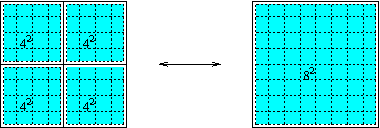
\includegraphics[width=3.75in]{coalesce.png}
\end{minipage}}
\FIGURE{Targeted refinement with backfill}{f:backfill}{
\begin{minipage}{6.15in}
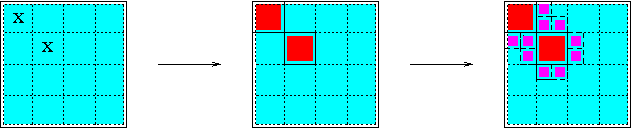
\includegraphics[width=6.15in]{kd-backfill.png}
\end{minipage}}



\FIGURE{
Coalesced patches proof-of-concept using a 2D cosmology density field projection.
\textbf{Left}: 2D cosmology density field projection.  
\textbf{Middle}: Balanced octree with 81701 patches.
\textbf{Right}: Balanced octree with 32529 coalesced patches. \\
}
{f:cosmo}{
\begin{minipage}{7.0in}
\begin{minipage}{2.2in}
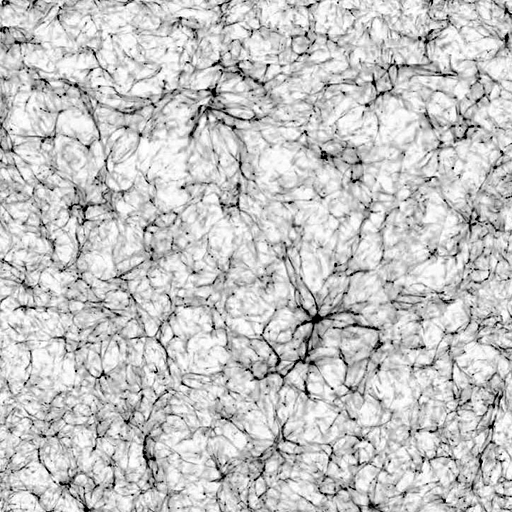
\includegraphics[width=2.2in]{cosmo2-invert.png}
\end{minipage} \ 
\begin{minipage}{2.2in}
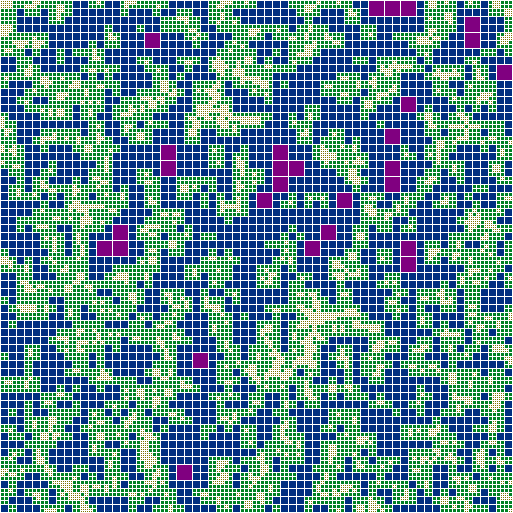
\includegraphics[width=2.2in]{cosmo2-4-1.png}
\end{minipage} \ 
\begin{minipage}{2.2in}
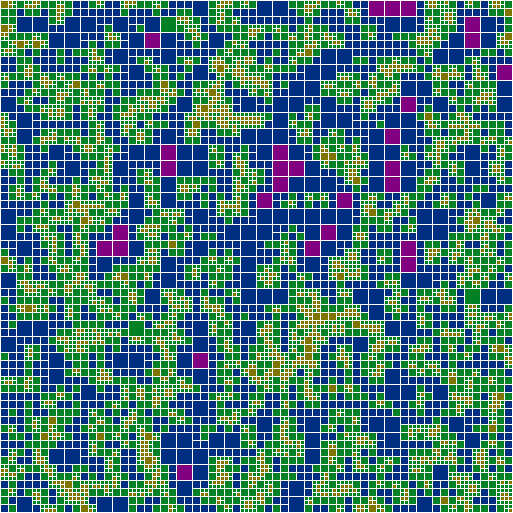
\includegraphics[width=2.2in]{cosmo2-4-2.png}
\end{minipage}
\end{minipage}
}


%-----------------------------------------------------------------------
\subsection{AMR data structure optimization: targeted refinement with backfill for ``deep'' AMR}
%-----------------------------------------------------------------------

\begin{verbatim}
AMR algorithm enhancements: targeted refinement by 4 or 8
   improves ``deep'' AMR
   refinement by 2 too ``shallow''
   back filling possible to regain effect of balanced tree
   sparse storage format of child patches to reduce storage 
   balancing octrees can have global effect
     balancing refinementy by 4 or 8 probabalistically (provably?) local
     no explicit AMR patches required for backfill--can live on child nodes 
     EXAMPLE: point refinement
\end{verbatim}

\begin{verbatim}
targeted refinement by 4 or 8
  especially effective for deep AMR, e.g. star formation with
    30+ levels
  still supports effective resolution jumps of 2 using backfill
patch coalescing
  reduced AMR overhead (number of patches) especially in shallow
    AMR relative to PARAMESH
  improved performance since locally unifrom grid instead of AMR
    patches
  still supports variable block sizes for optimizing memory
    hierarchy, parallel task size, task counts
variable patch resolution
instead of uniformly refining a patch, can replace with higher
  resolution array
need AMR machinery where resolution requirements change, not
  where high resolution is needed
\end{verbatim}

\FIGURE{
Targeted refinement proof-of-concept using multiple point sources in 2D.
\textbf{Left}: 2D point sources.  
\textbf{Middle}: Balanced octree with 2137 patches.
\textbf{Right}: Balanced octree with 158 explicit patches.
}
{f:dots}{
\begin{minipage}{7.0in}
\begin{minipage}{2.2in}
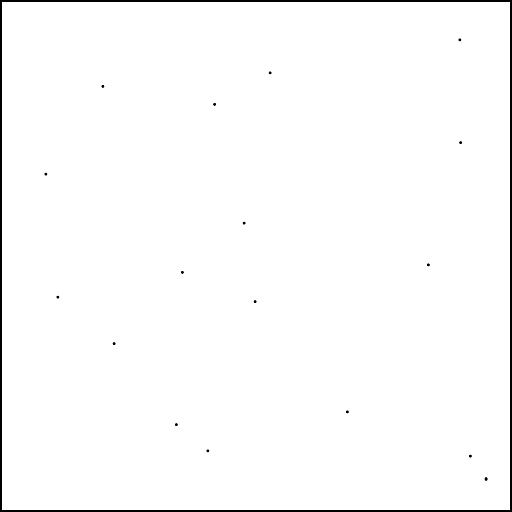
\includegraphics[width=2.2in]{dots-invert.png}
\end{minipage} \ 
\begin{minipage}{2.2in}
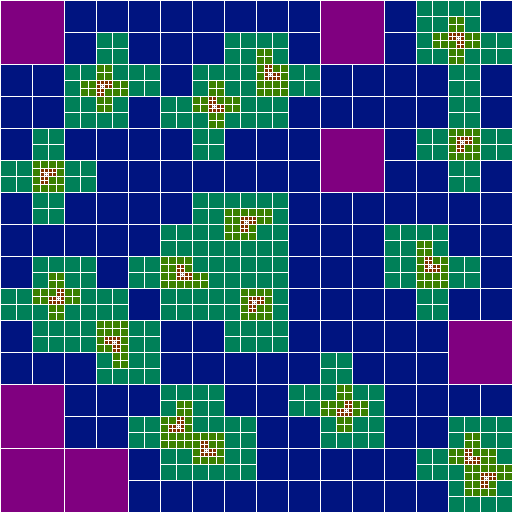
\includegraphics[width=2.2in]{dots-4-1.png}
\end{minipage} \ 
\begin{minipage}{2.2in}
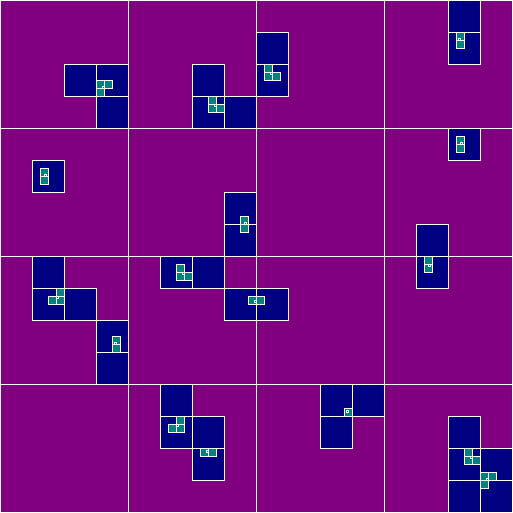
\includegraphics[width=2.2in]{dots-16-5.png}
\end{minipage}
\end{minipage}}

\begin{verbatim}
generalized octree-based AMR 
  8-tree, sparse 64-tree, sparse 512-tree
  decoupled AMR / Array
Fully distributed AMR data structure
For each local grid patch, only immediate neighbors and
  ancestors stored
  Proxies for remotely stored patches
    remote thread identifier + pointer
Store only actual data
  use flux registers for communication
  allocate patch ghost zones only for computation
Could store appropriate subset of neighbor data as well for
  fault-tolerance
AMR operations
  initial grid generation
  refinement criteria: tag refine or coarsen
  refinement or coarsening localized
\end{verbatim}


%=======================================================================
\section{CELLO IMPLEMENTATION} \label{s:implementation}
%=======================================================================


\begin{verbatim}
  Trac
  Subversion
  Languages
     C++, optional UPC, OpenMP
  User languages
     C++, C, Fortran, CUDA
  Parallel libraries / frameworks
     optional MPI (one-sided and send-recv), CHARM++
  testing
  documentation
\end{verbatim}
  
\section{DEVELOPMENT PLAN} \label{s:plan}

\begin{verbatim}
  CHARM++ generalized unigrid
     evaluate effectiveness
  AMR hyperbolic
  particle methods
  AMR elliptic
\end{verbatim}

\section{MILESTONES AND DELIVERABLES} \label{s:milestones}

\begin{verbatim}
   Cello software framework
   Complete Enzo II application
   large-scale demonstration using Enzo II
\end{verbatim}




\begin{verbatim}
 load balancing
    hierarchical
    load balance locally in given level
    different metrics at different levels
      memory at node level
      workload below
    different frequency at different levels
      lower frequency balancing at higher levels
         more costly
         solution changes less frequently
      higher frequency balancing at lower levels
         less costly
         solution changes more frequently
    task adjacency maintained
    use collected performance data
    explore overcompensation technique
       ala SOR
       two regimes
          local collapsing / explosion
          shock advancement
       identify regimes and adapt
    linearized morton curve / hilbert curve insufficient
       assumes equal work per patch
       particles are associated with nodes, changing weight
       adaptive timestepping drastically weights more highly  refined patches
       performance of physics algorithms on a patch is not necessarily uniform
          localized chemistry subcycling, front tracking, etc.
       arrays on patches may be different sized (assuming coalesced patches)
       linearization constricts dimensionality
          constrains data movement along a single dimension
          physics imbalances 4 dimensional
\end{verbatim}


\begin{verbatim}
dynamic scheduling
   task = grid patch + sequence of 
   dynamically schedule local tasks
      increased scheduling freedom
      improves slack for latency hiding
   schedule communication to/from local patches
   tasks scheduled biased towards patches that limit other patches, e.g. coarse
   optionally pipeline multiple methods on cores
      increase available parallelism: (e.g. deep AMR with many physics modules)
      helpful when multiple physics components available with similar costs
   communication scheduling to maximize releasing patches and prefetch data
   gang-scheduling groups of patches for improved GPU throughput / accelerator utilization

octree AMR versus SAMR   

other AMR libraries / frameworks
   Chombo
   PARAMESH
   SAMRAI

limitations of existing AMR libraries / frameworks

parallel scalability issues
   global synchronization / reductions
   load balancing
   I/O
   fault tolerance

AMR-specific parallel scalability issues
   elliptic
   remeshing--especially SAMR
   load balancing
   timestep determination

AMR datastructure scalability
   breadth--number of grid patches
   depth--range of multi-resolution
   floating point precision issues
   floating point range issues
   integer range issues

octree advantages
   arguably more scalable

octree limitations
   Morton ordering not always feasible
      different patch sizes
      different particle counts
      adaptive timestepping on finer levels
      physics method variations
         shock capturing--Riemann solver iterations
         variable subcycling of iterative stiff methods

hierarchical parallelism
   encourage communication within hardware components
      sockets within node
      cores within socket
      hyperthreads within core

parallel technology encapsulation / virtualization
  distributed / shared memory
    MPI (two-sided and one-sided) (distributed memory)
    OpenMP (shared memory) 
    UPC (either distributed memory or shared memory)
    CHARM++
  multiple strategies enhance software resiliency
    i.e. buggy MPI implementation--dynamically switch to UPC

hierarchical task scheduling
   multiblock (GPU)
   single block (process)
   plane / line (thread)

hybrid parallel
   MPI + OMP
   MPI + UPC
   UPC + OMP (?)
   CHARM++ + OMP (?)
   flexible subset of cores, sockets, nodes, supernodes
   Task scheduling CHARM++ model, but implemented in MPI, UPC, OMP
   processor-task affinity
software components
   functional decomposition
   ...
user functions supplied
   field / particle initialization
   particle advance
   particle computation
   particle - grid interaction
   block advance (multiple)
   inter-level flux correction
   refine / coarsen
   timestep determination
   constraint enforcement (div B)
   error checking / invariant checking for fault tolerance / software resiliency
      detects memory / cpu errors and mark core as faulty and bypass
relaxed local timestep control
   improves performance by not restricting timestep globally
   adaptive timesteps important for deep AMR runs, e.g. star formation (cite Abel)
   reducing global synchronizations and global dependencies crucial for extreme scaling
   allow variable timesteps within level
      eliminates requirement for global reduction
      timesteps quantized by two
         eliminates roundoff errors
      enforce timestep balancing--temporal level jumps(?)

distributed AMR hierarchy
   local patches: store parent, neighbors, children (sparse)
   not as memory efficient as globally stored nodes (3 pointers, 24 bytes average)
      cite (petascale AMR?)
   proxies for remotely stored patches
task migration
   migrate tasks dynamically
   CHARM++ model: pack, relocate, unpack data
   maintain locality by moving task to owner of a neighbor
   maintain parent-child locality when possible
      relax for deep hierarchies
   migrate using hierarchical parallelism

I/O
   parallel HDF5
   compression
   CRC error-checking and retry
   subset of nodes do I/O
   detection of faulty disk and mark as unusable
   different formats for different uses

fault-tolerance / software resilience strategies
   need to deal with continuous stream of failures
   MTTF < MTTC
   checkpoint to disk
      issue: failures will become more frequent than time to checkpoint
      agressively reduce checkpoint data size and write time
         dedicated I/O nodes
         compress
         check data
         methods identify which data modified
            may help lower disk output--only checkpoint modified data
   checkpoint to memory
     CHARM++ does this(?)
   detect hardware errors and mark as defective
       memory
       disk
       core
       socket
       node
       interconnect (pairs of nodes)
       software libraries (MPI versus UPC, etc.)
   flash memory
   log faults to disk for subsequent analysis
   performance resilience
      dynamically adapt to reduce cache thrashing / ineffeciency
          array blocking or padding in computational array registers
      adapt AMR patch size, refinement factor (2,4,8)
   fault-tolerant MPI
      FT-MPI
   leverage new approaches when available
      active research area
      keep up to date in latest practices
      design software to use new approaches

memory storage formats and data movement
   different formats for different uses
        optimized for storage
          option to not store guard / ghost cells
          AMR patches may be larger than computationally optimal
        optimized for computing
          store ghost cells
          improved data locality
          compute block size optimized for cache
             copied to array compute registers
             blocking/padding for cache / memory hierarchy
             groups of blocks for GPU / fp accelerators
   compute in reformatted ``computational registers''
      basic idea used in PARAMESH
         encapsulates functionality of both PARAMESH ``working block'' and ``work'' datastructures
      more flexible:
        arbitrary reordering of array axes
        arbitrary subset of axes
        arbitrary ghost zone depth
          more adaptable to existing legacy ``unigrid'' routines
          different reorderings possible for different methods (hydro, chemistry, etc.)
          flexibilty allows improved data-layout for single-thread performance
             cache blocking, padding
   communicate using reformatted ``flux registers''
      idea used in Chombo
   scheduler reuse for computation / communication scheduling

patch-local coordinates for particles
   control accumulation of roundoff
   minimize / eliminate effects of limited precision and range
   absolute coordinates computed when necessary
      analysis
      visualization

relative coordinates for patches   
   relative to neighbors
   computations frequently only require cell size and timestep
      hydrodynamics
   absolute coordinates computed dynamically when necessary to required precision
      initialization
      inline analysis
      global position dependent physics (materials)

global scaling of dx, dt?
   may not be needed
      only power-of-two quantization of dx, dt
        mantissa unchanged--no fp precision issue
        fp range issue
            support coordinate rescaling at deep levels
        
visualization
   use existing library, e.g. Visit
   Method can include visualization or inline analysis

software resilience
   take advantage of only Methods change data
   methods signal which fields / particles changed

particles
   groups of related particles stored together
   particles associated with grid patch
   flexibility in particle ownership
     may belong to immediate neighbor to reduce communication


problem scope
  hyperbolic conservation
     hydrodynamics
  elliptic problems
     self-gravity
  local physics
     chemistry
  elliptic support:
      global and level solves

AMR hierarchy data
     fields at multiple refinement levels (internal tree nodes as well as leaves)
       SEE PARAMESH user guide for motivation
       improving solution
       refinement criteria (cite Berger)
     fields only finest level (only tree leaves)
       reduced memory usage
       reduced computation: only finest level
       reduced communication: no inter-level interpolation (except refinement)

monitor: support for interfacing with user while running
   ``dashboard'' for real-time monitoring state of simulation
   
portal: support interfacing with other codes
   post-processing solvers
   data analysis pipeline
   visualization pipeline

automatic performance tuning
   computational block size, padding
   AMR patch size (by level)(possible?)
   refinement factor (2,4,8)
   load balancing frequency

application driven
   Enzo II
   cosmology / astrophysics
   requires wide range of AMR capabilities
     broad for galaxy structure formation
     deep for star formation
     turbulence
   requires wide range of physics capabilities
     hyperbolic: hydrodynamics
     elliptic: self-gravity, FLD radiation
     local physics: chemistry, heating/cooling
   decouple physics modules from AMR framework
   make both Enzo II and underlying AMR framework publicly available

testing
   lcatest: automated parallel application testing
   multiple test levels
      unit tests
      component tests
      application tests
      in-house / community beta-testing
         (progressive as functionality comes online)
   test for multiple things:
      functionality
      correctness
      performance
      scaling
   tests also help supplement user documentation
   use integrated performance monitoring
      PAPI for hardware counters
      PMPI for MPI communication
      new[] / delete[] overload for dynamic memory usage
         particularly important for AMR
      user-defined independent attributes
         cycle
         level
         process
      user-defined dependent metrics
         process-local patch counts
         process-local cell / zone counts
         process-local particle counts
      less frequent output at finer levels (more data)
   helps identify functional, performance, scaling bugs early
   extreme scaling designed into framework from the start

integrated performance monitoring
   summaries at different hardware levels
   less frequent at lower levels--more data
   more frequent at upper levels
   performance data available to other components
      load balancing based on actual memory usage / cpu time
      feedback for adaptivity
      help identify performance and scaling issues early
      poor-performance resilient

design
   still primarily in design phase
      available flexibility to modify current design
      little code and time wasted
   emphasis on thorough designing before coding
      prototype ideas before final implementation
      more time upfront known to lead to faster overall development times

upcoming systems
   BW
   ...
   ...
   core counts
   extrapolate top500 10 years
   what this means for extreme scalable AMR + particles

AMR basic unigrid
   unigrid is single AMR node(?)
     (how to link with level 1?)

I/O different output formats for different uses
   checkpointing
   analysis
   visualization
   general ``data dump''
   cheaper to rerun and regenerate data to process than dump and reread later
      inline analysis capability to reduce overall output required
   checkpoints
       node / processor independent: software resiliency
       checkpoints restartable on different configurations / platforms
   ``accessor code'' included with all output data

power -- idle components when not in use to reduce power usage
   shared caches help normalize performance

development
   implement progessively to fill user beta testing pipeline
\end{verbatim}

Petascale AMR research issue.

\pargraph{equation scope}

\begin{verbatim}
Nonlinear time-dependent hyperbolic conservation laws, and elliptic PDE's
synchronization and collective operations
parallel I/O
fault tolerance / software resiliency
distributed data structures
hierarchical memory
hierarchy parallelism
dynamic load balancing
heterogeneous computational components: GPU's
ease of use: unigrid update + interpolation + flux correction
weigh advantages / disadvantages of patch- versus tree-amr
\end{verbatim}


\section{Project Implementation}

\subsection{I/O}

\begin{verbatim}
Routines for data dumps, checkpointing, output of visualizaton /
  analysis
Leverage standard for AMR data output when possible
parallel HDF5
support I/O from subset of nodes , dedicated or shared, to
  optimize I/O performance, and overlap I/O with computation

\end{verbatim}

\subsection{Parallelism}

\begin{verbatim}
CHARM++ 
  data placement
  load balancing
  task scheduling
  checkpointing for fault tolerance
  performance monitoring and visualization
platform hierarchical architecture-aware data structures
  e.g. MPI communicator for cores in a socket, sockets in a
    node, nodes in a supernode, supernodes in a machine
  facilitates hierarchical dynamic load balancing
    improves dynamic mapping of data structures to hardware components
    E.g. load balance more frequently at core / socket level to
      keep functional units busy
    load balance node / supernode levels less frequently to keep
      memory usage uniform
    less frequent because:
      problem changes less at larger scales
      rebalancing is more expensive: larger data sizes, slower
        interconnects
    user-defined parameters and metrics for load balancing at
      different levels
      dynamically collected performance data can be fed back
        into hierarchical load balancing algorithm
  note linearization of octree datastructure is insufficient:
    assumes equal work per patch
    particles are associated with nodes, changing weight
    adaptive timestepping drastically weights more highly
      refined patches
    performance of physics algorithms on a patch is not
      necessarily uniform, e.g. localized chemistry subcycling, front
      tracking, etc.
    arrays on patches may be different sized
    linearization of patches reduces flexibility, and constrains data movement to a single dimension
\end{verbatim}

\subsection{Fault tolerance}

\begin{verbatim}
 FT-MPI 
  ``fault-tolerante MPI''
  http://icl.cs.utk.edu/ftmpi/overview/index.html 
MPICH-V 
  ``MPI Implementation for Volatile resources''
  http://mpich-v.lri.fr/index.php 
\end{verbatim}

\subsection{Software implementation}

\begin{verbatim}
Trac + SVN or mercurial
documenting as I go
OOP design: improves component reuse, controls software
  complexity, eases software maintenance
heavy emphasis on designing before coding
organize into components (subdirectories) of related classes
  Simulation, Control, Parallel, Task
  Amr, Patch: stores the AMR hierarchy
  Fields, Particles, Array: for storing data
  Block, Fluxes: for computing / communicating data
  Performance, Error, Parameters, Memory: globally-accesible functions; components in aspect-oriented programming paradigm; not sufficiently important to use AspectC, but techniques (primarily using templates) usable
  Method [Analysis] [Visualize]: hooks to user code; multiple methods permitted, selectable and scheduled at run-time
  External, User
interdependencies controlled at component and class level
classes with access functions used instead of raw arrays to improve modularity and modifiability
block structure for interface with user code
unit testing, including performance and parallel scaling
prototyping for proof-of-concept
application testing
code reviews
\end{verbatim}

\begin{verbatim}
Languages C++; user code can be C, C++, Fortran
attempt to componentize parallelization : MPI (two-sided, one-sided) + OMP + UPC + GPU + CHARM++
advantages / disadvantages of each
  MPI: + widespread, optimized implementations, familiar
  MPI: - data replication, difficult to use
  UPC + easier to use, combines shared memory view with efficient data affinity
  UPC - no concept of MPI communicator, still under development--not as mature
  OMP + can be used progressively
  OMP - not scalable outside of socket / node;  inefficiencies due to false cache sharing
  GPU + very fast / power efficient when usable
  GPU - no usable standard, difficult to program, difficult to map problem to hardware
  CHARM++ + higher-level, dynamic scheduling, dynamic load-balancing, fault tolerant through checkpointing to other node memory
  CHARM++ - requires learning separate language, separate runtime system, no data prefetching(?)
    currently not fully realizable for GPU since depends on
      computational code
    hierarchical parallelism: MPI + OMP, MPI + UPC, MPI + GPU,
      etc.
    advantages of hybrid
      reduced data replication from MPI distributed memory
      dynamic parallel threads--use more when helpful, fewer when not
      UPC
    disadvantages of hybrid
      performance hit from data sharing in MPI + OMP
      MPI and UPC communication cannot (currently) proceed concurrently
    code for two modes: distributed memory and shared memory
    parallel tasks: grid patches, arrays, grid patch groups,
      particle groups
    flexible data structure parameters (grid patch size, patch
      decomposition, patch grouping) to dynamically optimize task size
\end{verbatim}
    
%=======================================================================
\section{Enhancements}
%=======================================================================

\begin{verbatim}
Require more rigorous coding standards compared to Enzo
  development
Auto-tune where possible--automatically optimize for cache-,
  parallel-, vector-, solver-, etc. parameters
\end{verbatim}

%-----------------------------------------------------------------------
\subsection{Adaptive Mesh Refinement}
%-----------------------------------------------------------------------

\begin{verbatim}
enhancements for both ``deep'' and ``shallow'' AMR

Do not store a patch's global position, only local position
  relative to immediate neighbors, parent, and children. [Toward
  distributed AMR data-structure, and to address precision issues with
  deep AMR. Potential issues: boundary and initial conditions.] (see
  W013)
For very deep AMR where coarser levels never complete their
  timestep, delete coarse levels to free storage.
 Provide (or notify) neighboring patches with updated
  ghost zone data as soon as it's available.
 Support temporary ``allocate as-needed'' ghost zones
  in addition to ``permanent'' ones
Reduce tree-AMR node size by only storing parent, single
  neighbor, and single child. [Assuming one pointer for field data and
  SAMR patches indexed by single-precision offsets into parent
  patches, 32 bytes / tree-AMR and 48 bytes / patch-AMR]
Relax rigid refinement criteria to inhibit excessive changes in
  octree-like tree refinement.
Represent patch extents with (small) integer values relative to
  parent. [To reduce memory usage with deep AMR runs.] (see W012)
Support both structured AMR (Enzo-like) and tree-based AMR
Support flexible node types: memory-efficient versus
  compute-efficient.
\end{verbatim}

%-----------------------------------------------------------------------
\subsubsection{\code{Arrays} Component}
%-----------------------------------------------------------------------

\begin{verbatim}
Allow multiple root-level patches per MPI task. [To improve
  cache use for unigrid problems, and improve load-balancing for AMR.]
\end{verbatim}

%-----------------------------------------------------------------------
\subsubsection{\code{Control} Component}
%-----------------------------------------------------------------------

\begin{verbatim}
Reduce implicit dependencies by dynamically allocating parallel
  tasks, ala CHARM++.(e.g. currently Enzo loops through patches within
  a level, but a given patch can proceed as soon as it has all its
  boundary data)
Support optional uniform timesteps across all levels. [To
  improve parallel efficiency.]
Support optional variable timestep sizes within each level. [To
  reduce synchronization costs when computing global CFL condition.]
\end{verbatim}

%-----------------------------------------------------------------------
\subsubsection{\code{Storage} Component}
%-----------------------------------------------------------------------

\begin{verbatim}
Enforce strict control over data storage formats (e.g. files)
  (see W0009)
Require that all stored data be accessed through standard
  interface functions that are independent of specific file formats
  (i.e., stored datasets are conceptually treated as objects)
\end{verbatim}

%-----------------------------------------------------------------------
\subsubsection{\code{Fields} Component}
%-----------------------------------------------------------------------

\begin{verbatim}
User-controlled optional floor/ceiling limits on individual
  Fields (ala ``tiny\_number'' in Enzo), with user-specified Error
  behavior (warning, error, ignore, reset to given floor/ceiling,
  etc.)
\end{verbatim}

%-----------------------------------------------------------------------
\subsubsection{\code{Methods} Component}
%-----------------------------------------------------------------------

\begin{verbatim}
Integrate ``inits'' functionality into the main code
\end{verbatim}

%-----------------------------------------------------------------------
\subsubsection{\code{Parallelization} Component}
%-----------------------------------------------------------------------

\begin{verbatim}
Load-balance by having over-loaded processors reassign tasks to
  random processes. [To reduce global communication for determining
  which processes are under-loaded]
Load-balance using ``over-compensation'', since heavily-loaded
  processes tend to continue to become more heavily loaded (cosmology
  / star-formation application-dependent).
Only use inter-core, inter-cpu, inter-node, etc.
  level-communicators to bound communicator size and manage
  communication nonuniformity.
Support multiple (hybrid) and flexible parallelization
  strategies, including MPI-1 (2-sided send/recv), MPI-2 (1-sided
  get/put), OMP, and optionally UPC and GPU.
\end{verbatim}

%-----------------------------------------------------------------------
\subsubsection{\code{Parameters} Component}
%-----------------------------------------------------------------------

\begin{verbatim}
Support for user-supplied code for problem initialization.
\end{verbatim}

%-----------------------------------------------------------------------
\subsubsection{\code{Particles} Component}
%-----------------------------------------------------------------------

\begin{verbatim}
Store particle positions in single precision as -1 <= x,y,z <= 1
  relative to their containing patch. [To reduce storage, improve
  performance, and address precision issues with deep AMR.]
Use a binary tree data-structure to recursively partition the
  bounding boxes of particles.
\end{verbatim}

%-----------------------------------------------------------------------
\subsubsection{\code{Simulations} Component}
%-----------------------------------------------------------------------

\begin{verbatim}
Support ensembles within a single run, including inline-analysis

\end{verbatim}


%=======================================================================
\bibliography{papers}
\bibliographystyle{unsrt}
%=======================================================================

\end{document}

%==================================================================

